\section{Supervised Fine-Tuning: The Win That Was Not}\label{sec:sft}

The supervised fine-tuning (SFT) stage poses a single-variable question: does
response masking --- computing the loss only on response tokens, the standard
practice in instruction tuning --- improve a small reasoning-SFT recipe over
plain continued pre-training on the same data? The stage produced the study's
most instructive de-confound: an apparently significant 0.68-PPL win for
masking that turned out to be an artifact of scoring the two arms on different
token sets, and that collapsed to roughly a hundredth of a perplexity point
under a corrected protocol (Figure~\ref{fig:sft-confound},
Table~\ref{tab:sft}).

\paragraph{Setup.}
Both arms start from the faithful 1.19B-token base checkpoint and take one
pass over the same prepared OpenR1-Math reasoning corpus of 125{,}000{,}592
tokens, in the spirit of small-model reasoning distillation
\citep{xu2026vibethinker}: peak learning rate $5\times10^{-5}$ with cosine
decay to $8\times10^{-8}$, 5\% warmup, global batch 128 (micro-batch 4, 32
accumulation steps), AdamW \citep{loshchilov2017decoupled}, $n{=}3$ seeds per
arm (Table~\ref{tab:hparams}). The treatment applies a response mask; the
control is an iso-FLOP \texttt{--no\_mask} continued-pretrain arm that is
identical in data, ordering, schedule, steps, and token budget --- the loss
mask is the only variable. Because prompts are a small fraction of this
corpus, the masked arm takes loss on 97.6\% of tokens versus the control's
100\%; the treatment effect being tested is therefore the exclusion of a thin
prompt-token slice from the objective.

\paragraph{The advisory in-loop result.}
The in-loop evaluation (training-loop perplexity, not suite-stamped, $n{=}3$
seeds per arm) showed SFT at 11.595 versus the control at 12.273 --- a
$+0.679$ gap with a tight interval (95\% CI $[+0.676, +0.681]$) that would
read as a decisive win (Table~\ref{tab:sft}, top block). But the comparison is
confounded: each arm reused its own training mask at evaluation time, so the
SFT arm was scored on response tokens only while the control was scored on all
tokens. Perplexities over different token sets are not comparable numbers. The
in-loop verdict flagged this itself and capped the result to directional,
advisory-only, pending re-scoring under a shared protocol.

\paragraph{The corrected protocol.}
The verdict of record re-scores all seven checkpoints (base plus three seeds
per arm) on one fixed held-out response-masked reasoning set: 66 held-out
OpenR1-Math documents comprising 228{,}529 response tokens, produced by a
seeded document-level split with 13-gram deduplication against the training
set. On this common footing, base perplexity 14.127 falls to 11.573 (SFT) and
11.582 (control) --- improvements of 18.1\% and 18.0\% respectively --- and
the 0.68-PPL gap collapses to $+0.009$ PPL (95\% CI $[+0.0045, +0.0139]$,
$n{=}3$ seeds per arm), nominally significant but a small fraction of the
advisory number. A tokenizer-free full-sequence cross-check
on the same documents flips the sign: $-0.006$ PPL (95\% CI $[-0.011,
-0.001]$) with the control ahead, scored not significant under the
pre-specified one-sided improvement test. Since the masked and full-sequence
comparisons disagree, the recorded verdict is \emph{directional}: the two arms
are not yet separable. Across-seed spread on the held-out set is 0.001 PPL
within the SFT arm and 0.004 PPL within the control arm, so the ambiguity is
not seed noise --- the effect itself sits at the scale of the measurement.

\paragraph{Forgetting probe.}
Neither arm damages the base distribution. On a held-out FineWeb-Edu probe
\citep{penedo2024fineweb}, base perplexity 21.495 rises to 21.652 (SFT) and
21.660 (control), a $+0.7\%$ shift (Table~\ref{tab:sft}, bottom block). On the
standard suite (text-lm-v2, one representative seed per arm), wikitext-2 moves
from 37.010 to 37.082/37.084 against a noise floor of 1.304, and the code
corpus from 438.673 to 425.689/425.594 against a floor of 280.564 --- both
labeled retained/not significant. The three-seed confidence intervals in this
section apply to the in-domain reasoning set only; the standard-suite
retention numbers are single-seed spot checks.

\paragraph{Interpretation.}
The real effect at this scale is the \emph{data}, not the masking: continued
training on in-domain mathematical reasoning delivers essentially the entire
18\% perplexity gain, and excluding the 2.4\% prompt-token slice from the loss
adds at most a hundredth of a perplexity point of separation, of ambiguous
sign. The headline that response-masked SFT beats continued pre-training does
not survive an honest iso-FLOP control. The methodological point generalizes:
a comparison whose arms are scored on different token sets can manufacture an
apparent effect nearly two orders of magnitude larger than the corrected
estimate, while presenting a confidence interval tight enough to look
unimpeachable. The study's evidence gates treated the in-loop number as
advisory by construction; the fixed held-out set, defined once and shared
across all arms, is what the verdict rests on.

% tab_sft.tex -- SFT (response-masked) vs iso-FLOP --no_mask control vs base, with the confounded
% in-loop advisory numbers shown next to the corrected held-out re-score.
% Sources in Qwen3-0.6B/experiments/2026-06-27_qwen3-0.6b_sft-3seed/:
%   verdict.json (in-loop advisory, CONFOUND key), reasoning_verdict.json (corrected held-out + full-seq + forgetting),
%   eval/sft_seed0/suite_results.json + eval/ctrl_seed0/suite_results.json (standard suite, text-lm-v2), c5_evidence.json (recipe).
\begin{table}[t]
\centering
\caption{SFT at 596M: response-masked SFT vs.\ an iso-FLOP \texttt{--no\_mask} continued-pretrain control (identical data, LR schedule, and token budget; masking is the only variable) vs.\ the base.
Recipe: $\approx$125M OpenR1-Math tokens (one pass, 125{,}000{,}592 prepared), peak LR $5\times10^{-5}$ cosine $\rightarrow 8\times10^{-8}$, 5\% warmup, $n{=}3$ seeds per arm.
The in-loop comparison (top block) is \textbf{confounded --- advisory only}: the SFT arm was scored on \emph{response tokens only} while the control was scored on \emph{all tokens}, so its 0.68-PPL ``significant'' gap is not a like-for-like number.
Re-scored on one fixed held-out response-masked set (66 OpenR1-Math docs, 228{,}529 response tokens, 13-gram dedup vs.\ train), the gap collapses to $+0.009$ PPL; the exact tokenizer-free full-sequence cross-check flips sign ($-0.006$, control ahead, n.s.\ for improvement), so the masked and full-sequence comparisons disagree and the verdict of record is \emph{directional} (not-yet-separable), while both arms improve $\approx$18\% over base.
Seed spread within each arm: SFT $0.001$, control $0.004$ PPL.
Forgetting probe: held-out FineWeb-Edu PPL; wikitext-2/code retention is within the noise floor on the standard suite (\texttt{text-lm-v2}, representative seed).
Source files: \texttt{verdict.json}, \texttt{reasoning\_verdict.json}, \texttt{suite\_results.json}, \texttt{c5\_evidence.json} (2026-06-27 sft-3seed).}
\label{tab:sft}
\footnotesize
\begin{tabular}{lcccc}
\toprule
Evaluation (PPL, lower is better) & Base & SFT ($n{=}3$) & Control ($n{=}3$) & SFT $-$ Control (95\% CI) \\
\midrule
\multicolumn{5}{l}{\emph{In-loop advisory --- CONFOUNDED: SFT scored on response tokens, control on all tokens}} \\
In-loop train-window proxy & 14.262 & 11.595 & 12.273 & $+0.679$ $[+0.676,\,+0.681]$ (not comparable) \\
\midrule
\multicolumn{5}{l}{\emph{Corrected: one fixed held-out response-masked set (verdict of record)}} \\
Held-out masked reasoning PPL & 14.127 & 11.573 & 11.582 & $+0.009$ $[+0.005,\,+0.014]$ sig.\ \\
Full-sequence cross-check     & 14.713 & 12.067 & 12.060 & $-0.006$ $[-0.011,\,-0.001]$ n.s.\ (control ahead) \\
\midrule
\multicolumn{5}{l}{\emph{Catastrophic-forgetting probe (held-out FineWeb-Edu; higher $=$ more forgetting)}} \\
FineWeb-Edu PPL & 21.495 & 21.652 & 21.660 & retained ($+0.16$ vs.\ base, $\approx$0.7\%) \\
\bottomrule
\end{tabular}
\end{table}


\begin{figure}[t]
\centering
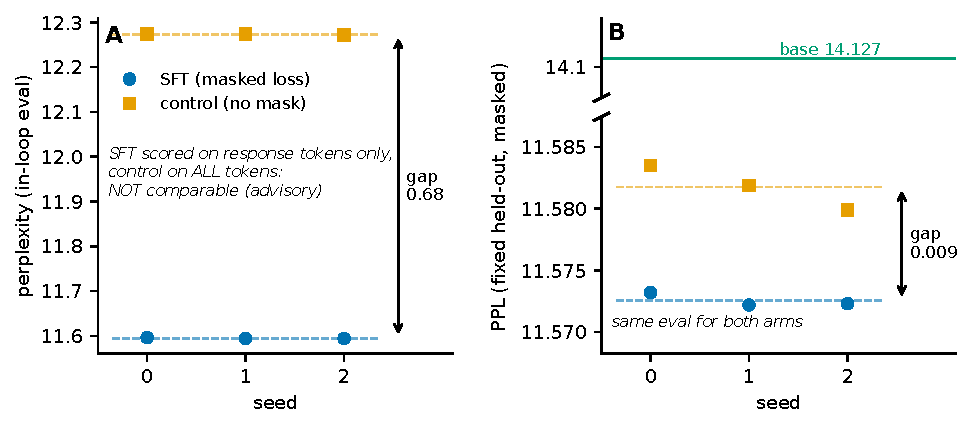
\includegraphics[width=0.9\linewidth]{figures/fig_sft_confound.pdf}
\caption{The SFT eval-token confound. Left: the in-loop advisory comparison
(training-loop perplexity, not suite-stamped) scores the SFT arm on response
tokens only and the control on all tokens, producing an incomparable
$+0.68$-PPL apparent gap (SFT 11.595 vs.\ control 12.273). Right: re-scored on
one fixed held-out response-masked set (66 OpenR1-Math documents, 228{,}529
response tokens, 13-gram dedup vs.\ train), the gap is $+0.009$ PPL (95\% CI
$[+0.0045, +0.0139]$) with a sign-flipping full-sequence cross-check
($-0.006$, n.s.) --- verdict directional. Budget: one pass over
125{,}000{,}592 OpenR1-Math tokens per arm, iso-FLOP, masking the only
variable; $n{=}3$ seeds per arm; across-seed spread SFT 0.001 / control 0.004
PPL. Source files: \texttt{verdict.json}, \texttt{reasoning\_verdict.json}
(2026-06-27 sft-3seed); rendered by \texttt{fig\_sft\_confound.py}.}
\label{fig:sft-confound}
\end{figure}
